
\documentclass{article}
\usepackage{hyperref}
\usepackage{graphicx}

\title{ LabWork10 Project - Kuwahara filter}
\date{}

\begin{document}
\maketitle

Nathan Choukroun labwork 10 project. 

Cuda programming of the Kuwahara filter on Google Colaboratory notebook. 

\section{Introduction}

The Kuwahara filter is commonly used in image processing to achieve noise reduction while preserving edges, producing a smoothing effect often described as painterly. The purpose of this project is to assess the performance of the Kuwahara filter on a GPU, both with and without shared memory optimization, to understand the advantages of parallelized processing. 

By reducing noise while maintaining sharp edges, it has applications in both artistic rendering and preprocessing for feature extraction in computer vision. However, the Kuwahara filter is computationally intensive due to the need to analyze multiple overlapping windows around each pixel.

The Kuwahara filter works by examining the neighborhood around each pixel. For a given pixel, four square windows are defined around it, each overlapping the pixel from a different direction. The brightness standard deviation is calculated for each window, and the window with the lowest standard deviation is selected. The pixel is then assigned the average color of that window, which effectively smooths the image in areas of low variance while preserving edges in high-variance areas.

The CUDA implementation of the filter assigns each pixel to an individual thread, where the RGB values of surrounding pixels are read directly from global memory. Each thread independently computes the standard deviation of brightness for the four windows around its designated pixel and selects the window with the lowest standard deviation. The pixel's color is then updated to the average RGB values of the chosen window. 

Shared memory is used to store pixel data for each thread block. Shared memory provides faster access than global memory, so by loading pixel values into shared memory once, multiple threads within a block can access this data without redundant memory loads. At the scale of data we are experimenting with, the time it takes to move all the data to memory adds up to make up longer times. Experiencing the same algorithm on super computers with and without shared memory may give different results. 

\section{Steps}

\begin{itemize}
    \item choose window size
    \item convert to hsv color
    \item loop the image grid
    \item select w size subwindows
    \item make the subwindow calculations
    \item find the variance of the subwindow
    \item compute the output pixel
\end{itemize}

\section{Results}

First test with a small image quality of 945x498 for a grid of 60x32
\begin{itemize}
    \item Time to run is: 0.9115
    \item Time to run is: 1.2930 (shared memory)
\end{itemize}

Result of the filter with the orginal image


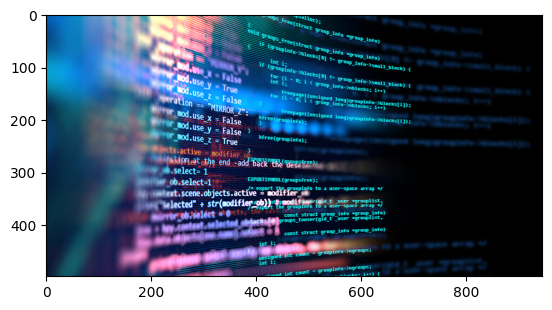
\includegraphics[width=0.6\textwidth]{code_plt.png}
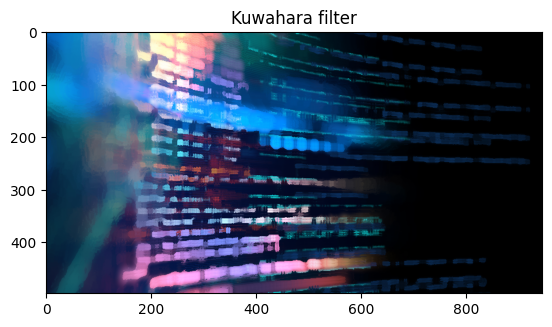
\includegraphics[width=0.6\textwidth]{code_plt_kuwahara.png}

Second test with a larger image of 1619x1080 for a grid of 102x68

\begin{itemize}
    \item Time to run is: 1.1561
    \item Time to run is: 1.5834 (shared memory)
\end{itemize}

Result of the filter with the orginal image


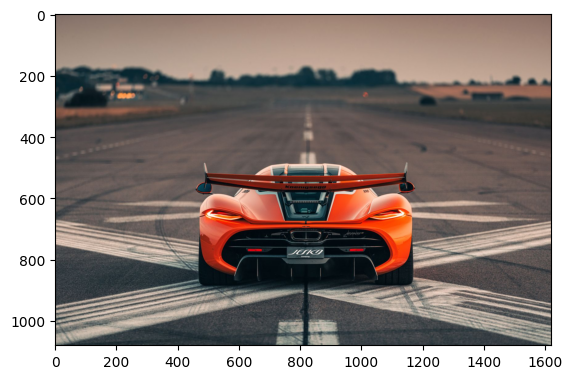
\includegraphics[width=0.9\textwidth]{jesko_plt.png}


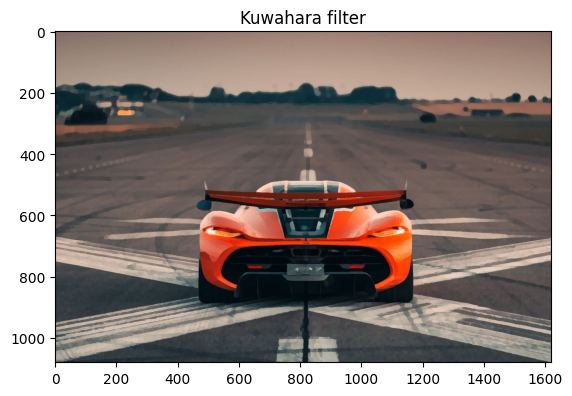
\includegraphics[width=0.9\textwidth]{jesko_plt_kuwahara.png}

\section{Conclusion}

These results show that shared memory isn't always the best choice, particularly for filters with limited memory access needs. Future work could explore other optimizations, like adjusting block sizes or testing different filter methods, to further improve performance. This project highlights that, in some cases, simpler memory access strategies can be more effective than complex optimizations, depending on the computer performances or specific tasks. 


\end{document}